\chapter{初段ミューオントリガーシステム}
本章では、ATLAS トリガーシステムの一つである初段ミューオントリガーシステムに着目し、Run-3におけるエンドキャプ部初段ミューオントリガーシステムについて述べる。

\section{ATLAS トリガーシステムの概要}
ATLAS実験では、LHCを用いて40MHzでの陽子陽子衝突の測定を行っている。しかし、データ記憶容量の制限が存在するためすべての衝突事象を保存することはできず、現在の制約では記憶するトリガーレートを約1kHzまで削減する必要がある。
そのため、物理として興味のある事象のみを効率よく取得するトリガーシステムを用いて事象選別を行う。

ATLAS 検出器では、ハードウェアにより高速にトリガー判定を行う初段の Level-1 Trigger (L1 Trigger)、ソフトウェアで詳細なトリガー判定を行う後段の High-Level Trigger (HLT) で構成される2段階のトリガーシステムを用いている。

\begin{figure}[tb]
  \centering
  \rule{8cm}{6cm}
  %\includegraphics[clip, width=14cm]{}
  \caption{ATLAS トリガーシステムの全体像}
  \label{fig:fit_def}
\end{figure}

\subsubsection{Level1 Trigger}
初段トリガーである Level-1 Trigger では、ATLAS 検出器から送られてくる40MHzの衝突事象を2.5 $\mu s$ 以内にトリガー判定を行い、イベントレートを100 kHzまで落とす必要がある。このような高速でのデータ処理を行うために、L1 Trigger は Application Specific Integrated Circuit (ASIC)や Field Programmable Gate Array (FPGA) で構成されるハードウェアに実装されている。
ASIC と FPGA は




・L1Calo\\
・L1Muon\\
\begin{figure}[tb]
  \centering
  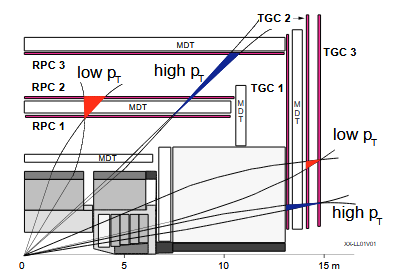
\includegraphics[clip, width=10cm]{fig/3/muon_trigger_overview.png}
  \caption{初段ミューオントリガーに用いる検出器の設置位置}
  \label{fig:muon}
\end{figure}

・Central Trigger
\subsubsection{High-Level Trigger}


\section{Run-3におけるエンドキャプ部初段ミューオントリガー}

\subsection{トリガーセクター}
ROIの話
\begin{figure}[tb]
  \centering
  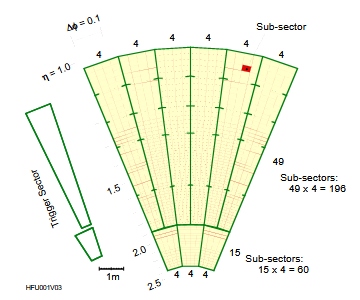
\includegraphics[clip, width=10cm]{fig/3/RoI.png}
  \caption{RoI}
  \label{fig:RoI}
\end{figure}


\subsection{ミューオンの運動量の算出}
運動量の算出の話
\begin{figure}[tb]
  \centering
  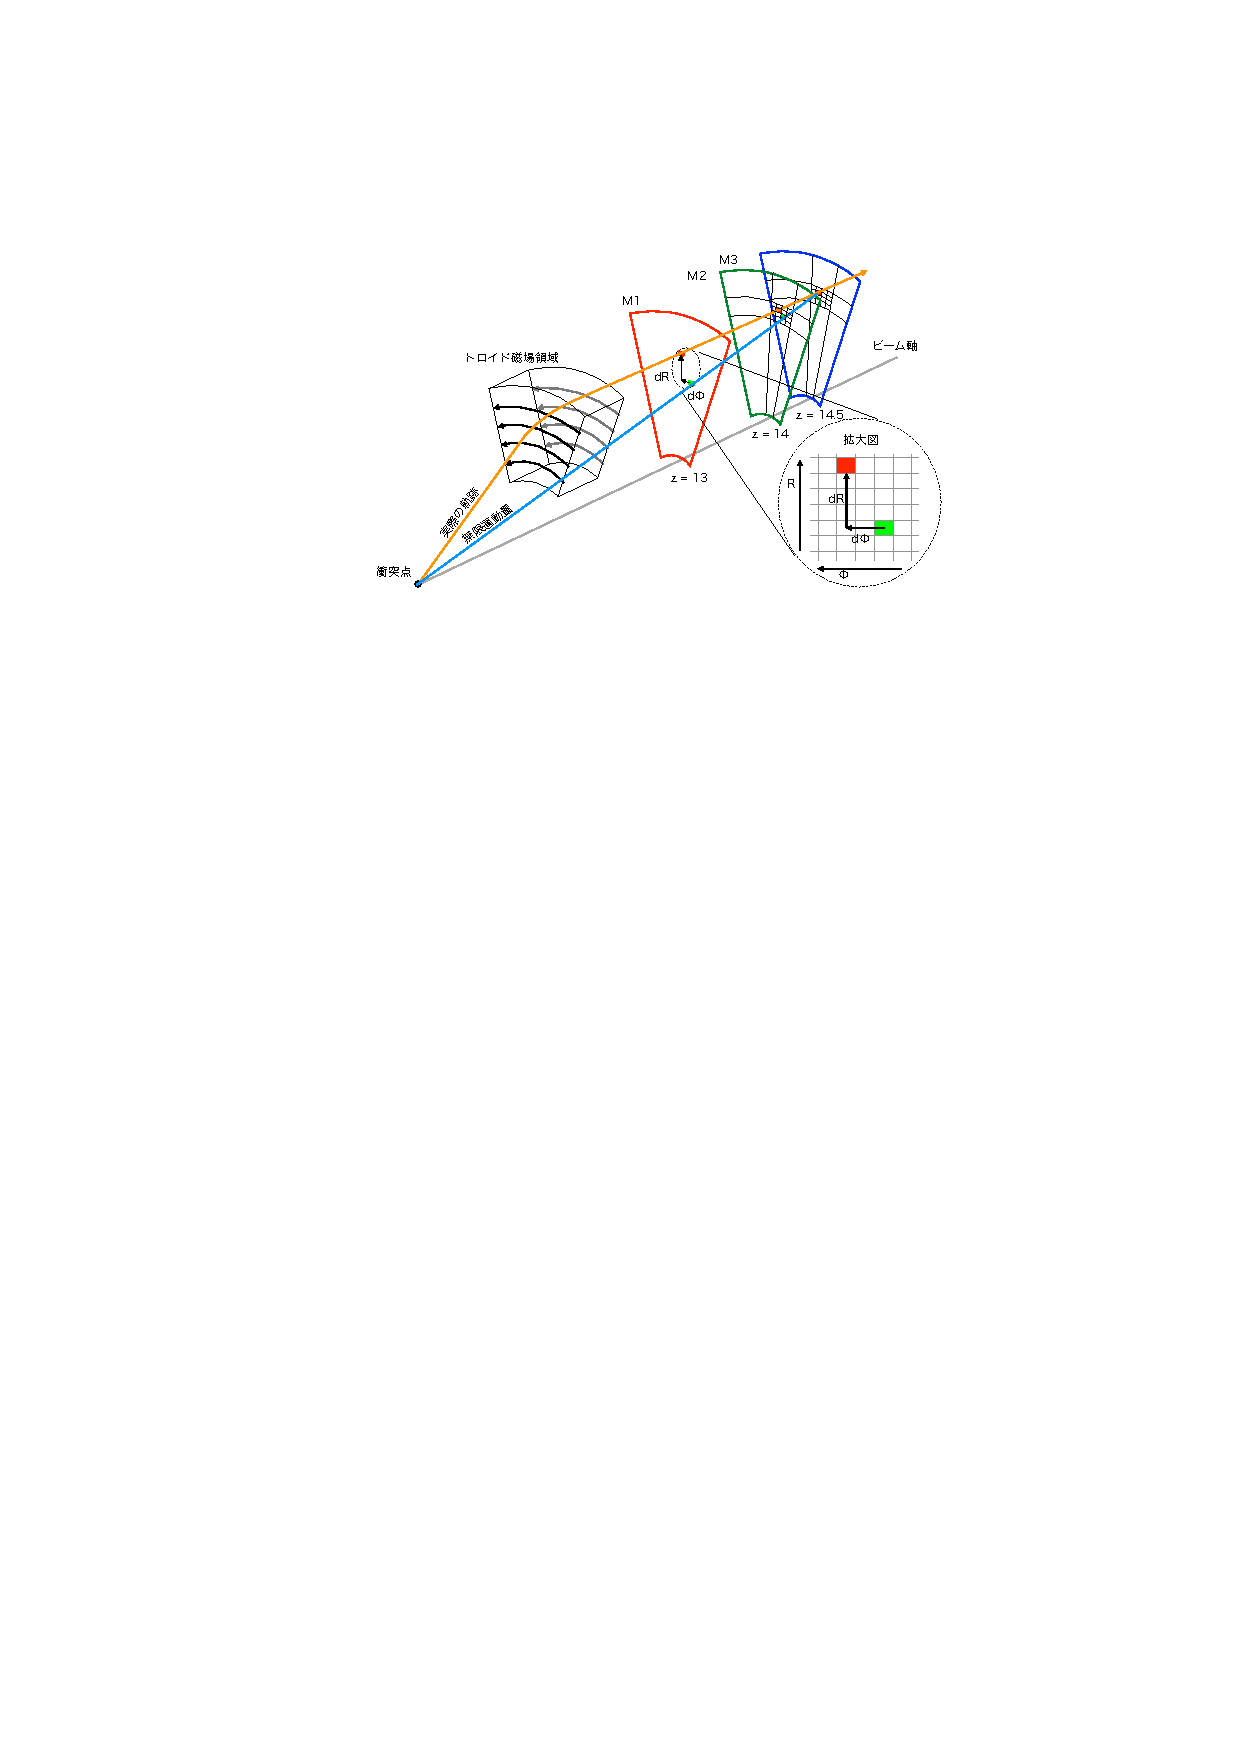
\includegraphics[clip, width=14cm]{fig/3/akatsuka_mt_trigger_scheme.pdf}
  \caption{ATLAS検出器エンドキャップ領域におけるトリガースキームの概念図\cite{article:akatsuka-mron}。無限大の運動量を持つミューオンを仮定し、磁場によって曲げられたミューオンとの位置の差を用いて$\pt$を計算する。}
  \label{fig:trigger-scheme}
\end{figure}

\subsubsection{Coincidence Window (CW)}
・CWの話
・現行CWの作成手法

\subsection{エレクトロニクス}

\section{2022年 Run-3 における初段ミューオントリガーの性能}
・Efficiency
・Rate

・電荷
・位置
・問題点


\subsubsection{Run-2における最適化手法}
・検出器のズレ<Run-2での検出器のズレの測定図>
\begin{figure}[tb]
  \centering
  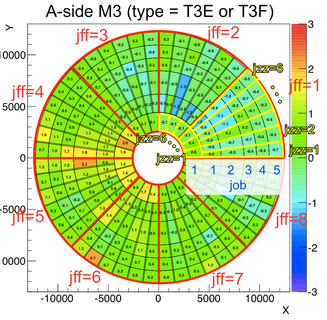
\includegraphics[clip, width=10cm]{fig/4/zure.png}
  \caption{Run-2での検出器のズレの測定図}
  \label{fig:Resolution}
\end{figure}
・検出器アライメント
<山内さんの手法>
<木戸さんの手法の説明>


\section{本研究の目的}


Run-3における初段ミューオントリガーの性能を向上させるために、現状では上記で述べた最適化手法を行う必要がある。しかし、Run-2で行われていた最適化手法は、各CWごとに1マスずつ6段階の閾値を確認する手法のため膨大な作業量が必用である。

・作業量が膨大
・機械学習に注目














